\chapter{Context of the work}
\minitoc
\newpage

\setcounter{secnumdepth}{0} % Set the section counter to 0 so next section is not counted in toc
% ----------------------- Introduction ----------------------- %
\section{Introduction}
This chapter introduces the general context of this report.
I start by presenting the frame of the project as well as the host company.
Then comes the enumeration of the problems which led to the realization of the project.
I wrap it up by defining the methodology I've followed to carry out my work.

\setcounter{secnumdepth}{2} % Resume counting the sections for the toc with a depth of 2 (Sections and sub-sections)

\section{General framework of the internship}
This project was carried out within the frame of obtaining an Engineering Degree in the domain of Networking and Security at the IT Business School (ITBS).
The internship took place fully remotely at Navoy for five months starting from the 26th of January 2022 to the 30th of June 2022 with the purpose of further developing an existing AI travel technology platform as well as migrating its infrastructure for scalability and to adhere to modern DevOps principles.

% ----------------------- Company overview ----------------------- %
\section{Company overview}
This section introduces the host company {\bf Navoy} as well as the services it offers.
\subsection{About Navoy}
"Navoy is an AI Travel Technology that allows you to craft and book ultra personalized trips with seamless automated AI flow." \cite{about-navoy}
\begin{figure}[H]
  \centering
  \makebox[\textwidth]{
\includegraphics[width=10cm]{src/assets/images/navoy-logo.png}}
  \caption{Logo of Navoy}
  \label{fig:logo-of-navoy}
\end{figure}

\subsection{Navoy's services}
\subsubsection*{\underline{Customized Itineraries}}
Navoy enables travel agents to generate trip itineraries with any level of customization in no time, with just a few clicks. The platform leverages AI technology to create highly personalized travel experiences.

\subsubsection*{\underline{Trip Management}}
The platform offers a simple and efficient system for managing itineraries, flights, and accommodations in seconds. Users can modify generated trips manually in a seamless way if they would like to add their magical touch to their trip.

\subsubsection*{\underline{All Destinations \& Experiences}}
Navoy provides expert knowledge on all destinations around the globe and recommendations for the most relevant local experiences and activities. Trips can be exported as offline PDFs for convenience.

\subsubsection*{\underline{Enterprise Solutions}}
For businesses, Navoy offers API access to huge travel databases from vetted hotels to personalized activities and attractions, allowing companies to streamline personalized and automated AI trip planning into their business flow.

% ----------------------- Stating the problem ----------------------- %
\section{Stating the problem}
Navoy -having ambitious goals to scale their AI travel technology platform over the next 2 to 4 years- wants to enhance their existing system to handle increased traffic and provide more personalized travel experiences. As the travel industry rebounds post-pandemic, there's a growing demand for automated, personalized trip planning solutions. The current monolithic architecture of Navoy's platform faces scalability challenges and needs modernization to support enterprise-level API access and real-time travel data processing. The company seeks to migrate to a microservices architecture while maintaining the seamless user experience that defines their AI-powered travel planning platform.

% ----------------------- Assessment of the case ----------------------- %
\section{Assessment of the case}
\subsection{Describing the work procedure}
The work on any project must first of all be preceded by a thorough study of the existing ones which undermines the strengths and weaknesses of the current system, as well as the business decisions that should be taken into account during the conception as well as the realization.
\subsection{Criticizing the current state}
After studying the existing, we can determine its limitations:
\begin{itemize}
  \item Monolithic architecture limits independent scaling of different platform components.
  \item Real-time travel data processing faces bottlenecks during peak usage periods.
  \item Enterprise API access requires manual intervention for onboarding new business clients.
  \item Current infrastructure lacks comprehensive monitoring and logging capabilities.
  \item Development deployment cycles are slow, hindering rapid response to user feedback and market changes.
\end{itemize}
\subsection{Proposed solution}
The solution to these problems is refactoring the whole application to separate sub-applications or microservices where the AI recommendation engine, trip management, and booking processes can be scaled independently of the other parts of the application.
This way, it will be easier to maintain and scale the different services as well as respond faster to issues and know exactly what caused them in the first place.
I of course have to create and organize the deployment pipelines from start to finish in addition to creating any hardware or software resources that I need for the deployment in the cloud.
I also suggest going further by adding recent monitoring solutions for all of the infrastructure in order to increase the availability and the reliability of the application and ultimately improve the experience of the clients using Navoy.

\newpage

% ----------------------- Development Methodology ----------------------- %
\section{Development Methodology}
\subsection{Agile methodology}
Agile is a structured and iterative approach to project management and product development.
It recognizes the volatility of product development, and provides a methodology for self-organizing teams to respond to change without going off the rails.

\subsection{Scrum methodology}
Scrum teams commit to completing an increment of work, which is potentially shippable, through set intervals called sprints.
Their goal is to create learning loops to quickly gather and integrate customer feedback.
Scrum teams adopt specific roles, create special artifacts, and hold regular ceremonies to keep things moving forward.

\subsection{Kanban methodology}
Kanban is all about visualizing your work, limiting work in progress, and maximizing efficiency (or flow).
Kanban teams focus on reducing the time a project takes from start by using a Kanban board to continuously improve their flow of work.
To explain more in details, Kanban is based on a continuous workflow structure that keeps teams nimble and ready to adapt to changing priorities.
Work items —represented by cards— are organized on the board where they flow from one stage of the workflow or column to the next.
Common workflow stages are To Do, In Progress, In Review, and Done.

\subsection{The choice for Navoy}
Since this project involves developing and scaling an AI travel platform that needs to adapt to changing travel industry demands and user preferences, I chose to use Agile methodology with 1-week sprints. This approach provides the perfect balance between structure and flexibility, allowing for rapid iterations and quick response to feedback while maintaining clear development goals and milestones.

The 1-week sprint cycle enables me to deliver incremental improvements to the platform while ensuring that any changes in requirements or priorities can be accommodated without significant disruption to the development process.

\begin{figure}[H]
  \centering
  \makebox[\textwidth]{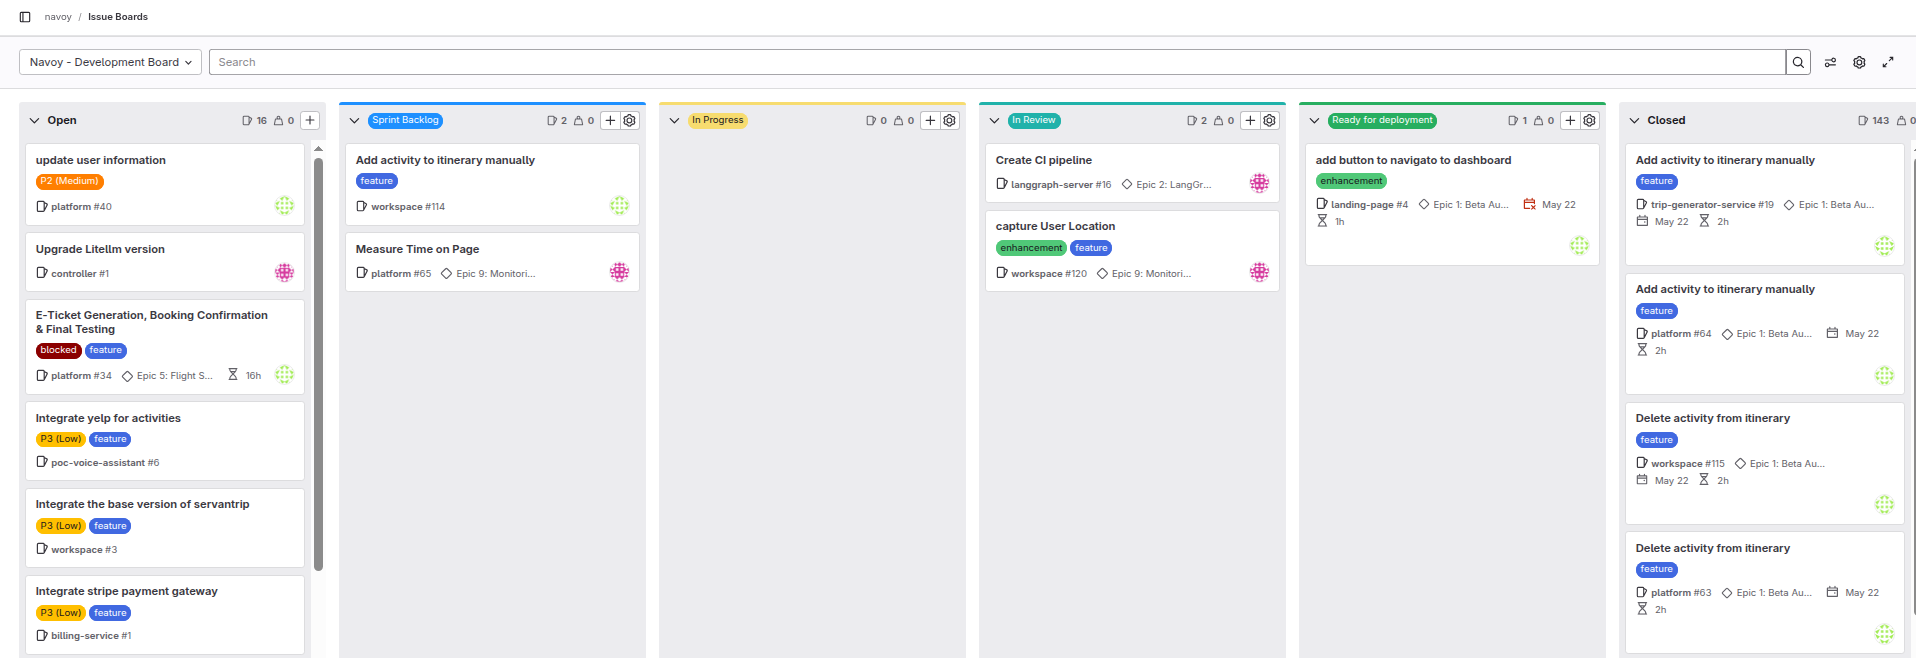
\includegraphics[width=\linewidth]{src/assets/images/navoy-board.png}}
  \caption{Navoy project Sprint board}
  \label{fig:navoy-project-sprint-board}
\end{figure}

\subsection{Unified Modeling Language}
The Unified Modeling Language (UML) is a general-purpose, developmental, modeling language in the field of software engineering that is intended to provide a standard way to visualize the design of a system. In my case, I used UML to design the top level view of the systems therefore I only used the Use Case and Sequence diagrams.

\setcounter{secnumdepth}{0} % Set the section counter to 0 so next section is not counted in toc
% ----------------------- Conclusion ----------------------- %
\section{Conclusion}
In this chapter, I presented not only the host organization but also the general context of the project and why it's needed.
I then criticized the current state of the Navoy application and discussed the possible development methodologies.
Lastly, I picked the most ideal choice for me which is Agile with 1-week sprints.
